% Chapter Template

\chapter{Code} % Main chapter title

\label{Chapter3} % Change X to a consecutive number; for referencing this chapter elsewhere, use \ref{ChapterX}

%----------------------------------------------------------------------------------------
%	SECTION 1
%----------------------------------------------------------------------------------------

%\section{Code organisation}

The code I have developed for this project is all publicly available on my github page (\cite{FB}). It can easily be installed using the setup file provided, which makes it easy to then use Python's customary import command to play with the code.
The code is organised in several sub modules and makes use of factories in plenty of places so that I can easily try out different puzzles, dimensions, search techniques, heuristics, network architecture, etc... without having to change anything but configuration or parameter in the command line. Here is a visual overview of the code base with the main dependencies between the main submodules and classes:

\begin{landscape}
\begin{figure}[H]
\centering
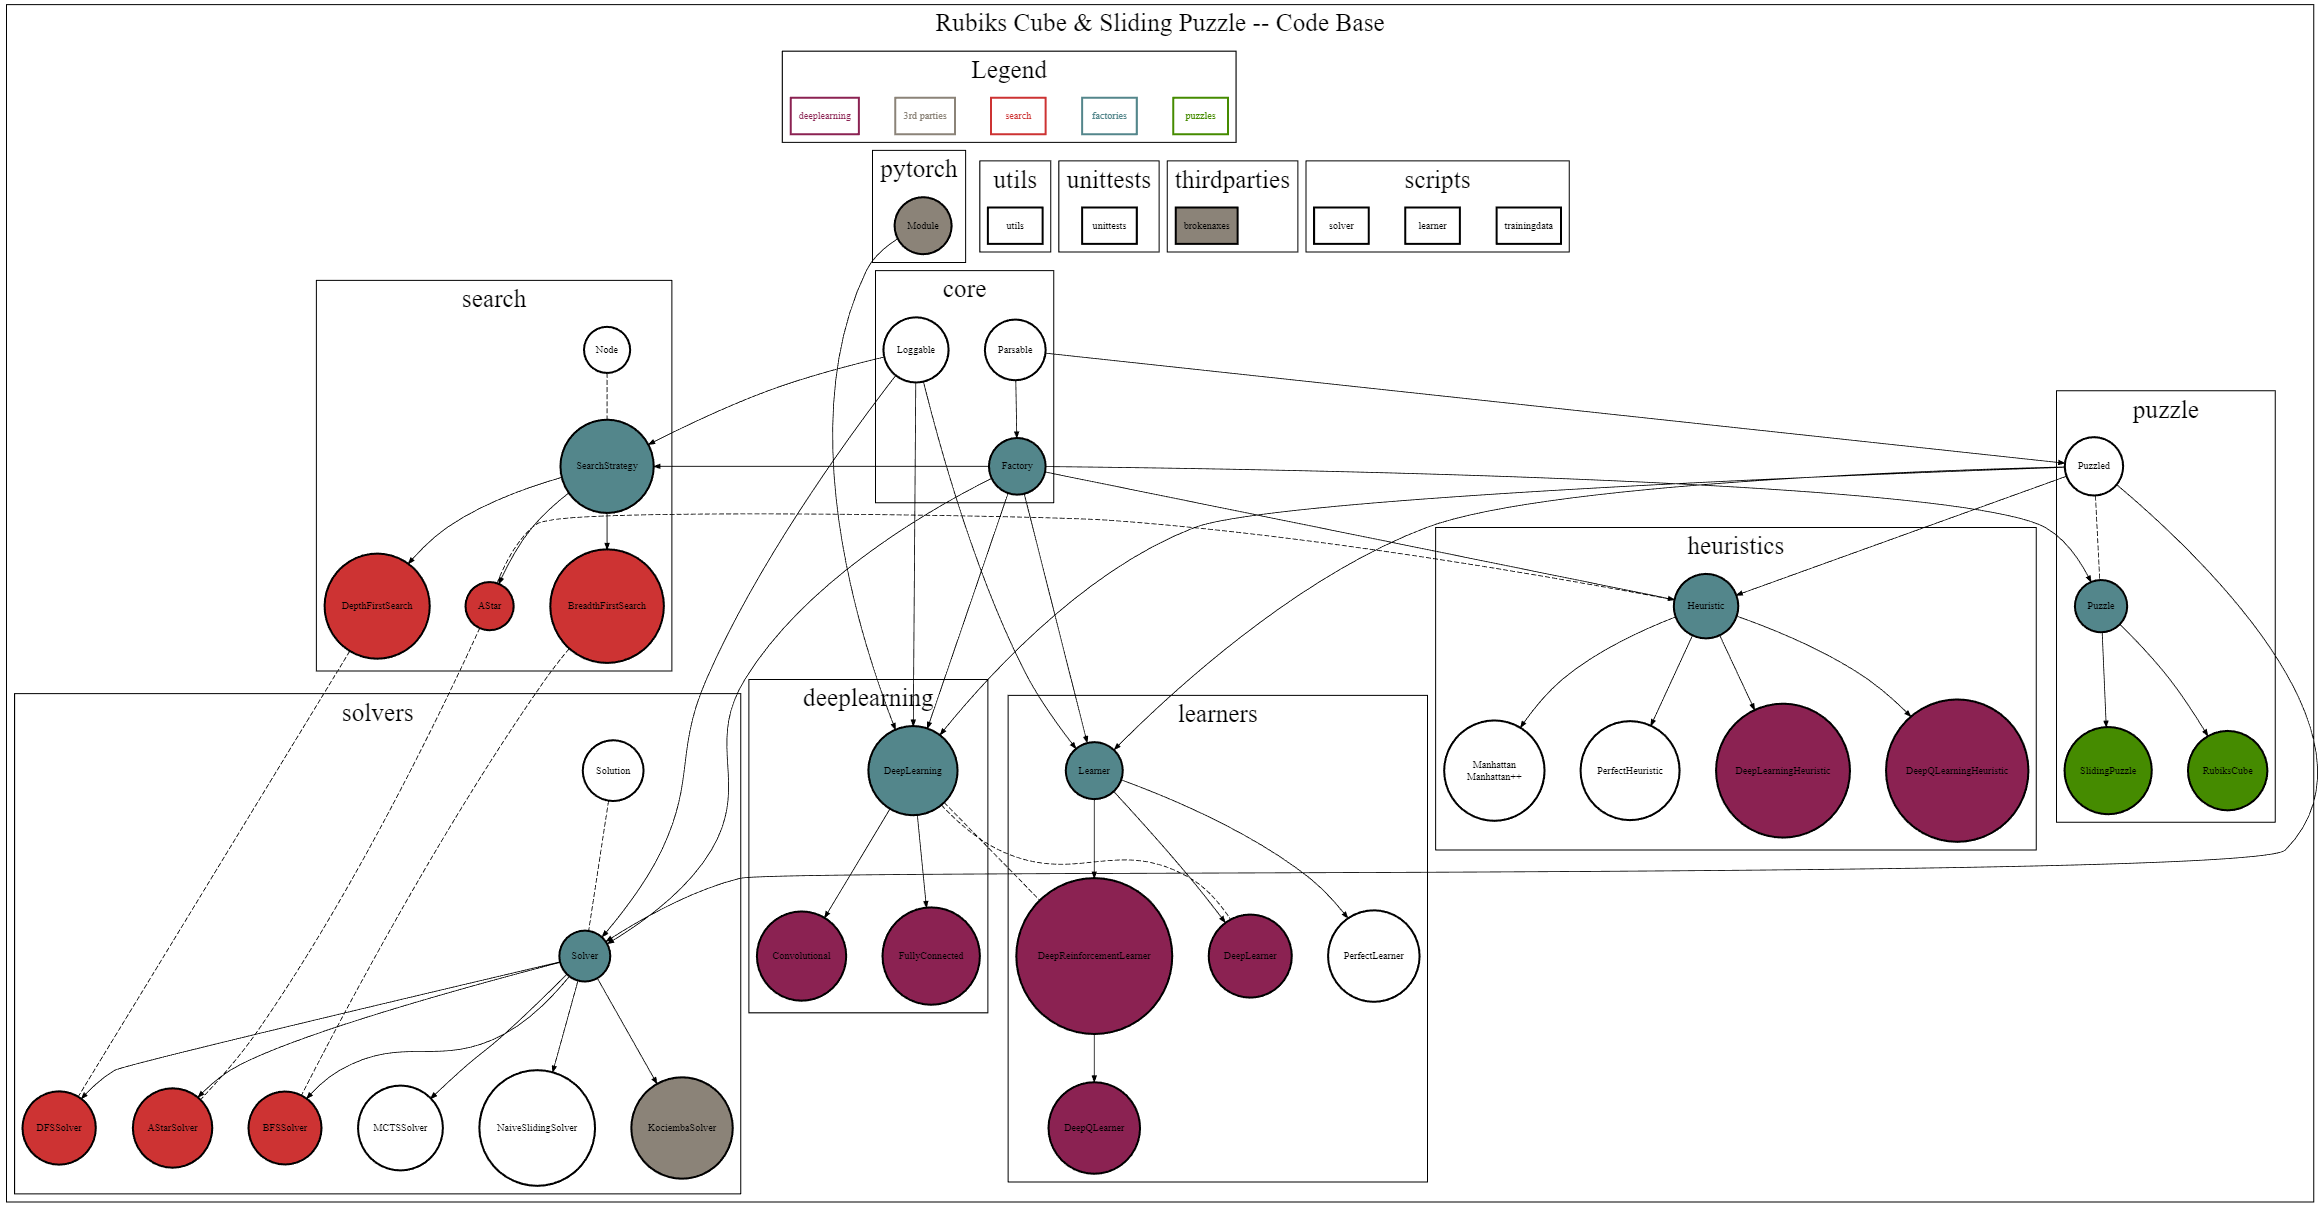
\includegraphics[scale=0.5]{./Figures/codebase}
%\decoRule
\caption[Codebase]{Code base}
\label{fig:Codebase}
\end{figure}
\end{landscape}


Let me describe what each submodule does:

\section{rubiks.core}
This submodule contains base classes that make the code base easier to use, debug, and extend. It contains the following:
\begin{itemize}
\item Loggable: a wrapper around Python's logger which automatically picks up classes' names at init and format things (dict, series and dataframes in particular) in a nicer way.
\item Parsable: a wrapper around ArgumentParser, which allows to construct objects in the project from command line, to define dependencies between object's configurations and to help a bit with typing of configs. The end result is that you can pretty much pass **kw\_args everywhere and it just works.
\item Factory: a typical factory pattern. Concrete factories can just define what widget they produce and the factory will help construct them from **kw\_args (or command line, since Factory inherits from Parsable)
\end{itemize}

\section{rubiks.puzzle}
This submodule contains:
\begin{itemize}
\item Puzzle: a Factory of puzzles. It defines states and actions in the abstract, and provides useful functions to apply moves, shuffle, generate training sets, tell if a state is the goal, etc. Puzzle can manufacture the two following types of puzzles:
\item SlidingPuzzle. Implements the states and moves of the sliding puzzle.
\item RubiksCube. Implements the states and moves of the Rubik's cube.
In addition, in contains a Puzzled base class which most below inherit from. That allow e.g. heuristics, search algorithms, solvers and learners to know what puzzle and dimension they operate on, without having to reimplement these basic facts in each of them.
\end{itemize}

\section{rubiks.search}
This modules contains graph search strategies. I have actually reused the code I implemented for one of the AIPnT assignments. It contains the following classes:
\begin{itemize}
\item Node: which contains the state of a graph, as well as link to the previous (parent) state, action that leads from the latter to the former and the cost of the path so far.
\item SearchStrategy, a Factory class which can instantiate the following three types of search strategies to find a path to a goal:
\item BreadthFirstSearch, which is obviously an optimal strategy, but not particularly efficient.
\item DepthFirstSearch, which is not an optimal strategy, and also generally not particularly efficient.
\item AStar, which is optimal, and as efficient as the heuristic it makes use of is.
\end{itemize}

\section{rubiks.heuristics}
\label{HSS}
This module contains base class Heuristic, also a Factory. Heuristic can instantiate the following heuristics, which we can use in the AStar strategy from the previous section:
\begin{itemize}
\item Manhattan: at current time of writing, this is specific to the SP and will be discussed in more details in \ref{S33},
\item PerfectHeuristic: this reads from a data base the optimal costs, pre-computed by the PerfectLearner (see below \ref{PLcode})
\item DeepLearningHeuristic: this uses a network which has been trained using DRL by the DeepReinforcementLearner (see below \ref{DRLcode})
\end{itemize}



\section{rubiks.deeplearning}
This module is a wrapper around Pytorch. It contains:
\begin{itemize}
\item DeepLearning: a Puzzled Loggable Factory that can instantiate some configurable deep networks, and provide the necessary glue with the rest of the code base so that puzzles be seemlessly passed to the networks and trained on.
\item FullyConnected: wrapper around a Pytorch fully connected network, with configurable layers and size.
\item Convolutional: tdb
\end{itemize}


\section{rubiks.learners}
\label{PLcode}
\label{DRLcode}
This module implements learners, which learn something from a puzzle, store what they learnt, and can display interesting things about what they learnt.

\begin{itemize}
\item Learner is a Puzzled Loggable Factory. It provides some common code to learners (to save or purge what they learnt), kick off learning and plot results. Concrete derived implementation define what and how they learn, and what interesting they can display about this learning process. Currently the two implemented learners are:
\item PerfectLearner: It instantiates an optimal solver ($A^{*}$ with a configurable heuristic - but will only accept heuristic that advertise themselves as optimal. The learning consists in generating all the possible configuration of the considered puzzle, solve them with the optimal solver, and save the optimal cost of it as well as those of the whole solution path. The code allows for parallelization, stop and restart so that we can run on several different occasions and keep completing a database of solutions if necessary or desired. Once the PerfectLearner has completed its job, it can display some interesting information, such as the puzzle's God's number, the distribution of number of puzzles versus optimal cost, the hardest configuration it came across, and how long it took it to come up with the full knowledge of that puzzle. I will show in section \ref{PLSS} how to run an example. Notice that for puzzles of too high dimension, where my computing resources will not allow to solve exhaustively all the configurations of a given dimension, this class can still be used to populate a data base of optimal costs, which can then be used by DeepLearner. If it is to be used this way, the PerfectLearner can be configured to use perfectly random configurations to learn from, rather than going through the configurations one by one in a well defined order.

\item DeepLearner tbd
\item DeepReinforcementLearner: It instantiates a DeepLearning (network), and trains it using DRL. It then saves the trained network, which can then be used in the DeepLearningHeuristic we have seen earlier in section \ref{HSS}. The


\end{itemize}


\section{rubiks.solvers}
This module implements solvers, which solve puzzles. The base class Solver is a Factory of solvers, and in addition to being able to instantiating the following types of solvers, can run different solvers through a similal sequences of random puzzles (for various increasing degrees of difficulty (shuffling), and/or perfectly shuffled ones) and display a comparison of how they perform in a number of metrics.

\begin{itemize}
\item DFSSolver
\item BFSSolver
\item AStarSolver
\item NaiveSlidingSolver
\end{itemize}

\section{rubiks.scripts}


Finally it is worth noting that the code will save on disk a lot of data (e.g. the learners will save what they have learnt, e.g. a Pytorch network or a data base of optimal costs, the performance comparison will run solvers versus very many configurations of puzzles and save the results for later being able to display) etc... The base of the tree to save all this data can be chosen by setting up the "RUBIKSDATA" environment variable. If not, it will go somewhere in you HOME :)
